
\section{Participation in rhythmic events}

As a component of exploratory play, we are interested in giving our
robot the ability to participate in patterned activity in real time
with a human partner.  We include in principle any form of
coordinated motor activity, including vocalization
(singing, proto-dialogue), and gesturing (tapping, dancing).
%
For example, if a human starts humming or tapping something rhythmic, 
we'd like the robot to rapidly join in.

Why is this useful?  Participation in rhythmic activity is a means to
an end, rather than a goal in itself.  The overall goal is to make
machine learning on our robots more autonomous.
%
Knowing the overall structure of an activity gives a ``skeleton'' upon
which the specific objects and actions (potentially initially
unmodeled) within that activity could be analysed.
%
Also, participating in activity is better than just observing it,
since there is an implicit signalling of ``comprehension'' level
available to the human partner, who can reasonably be expected to
adjust their behavior accordingly.


\subsection{Mechanism}

The theoretical mechanism was reported in deliverable 1.6.
We now describe the outcome of a practical application
of that mechanism to vocal interaction.


\begin{figure}[hbt]
\centerline{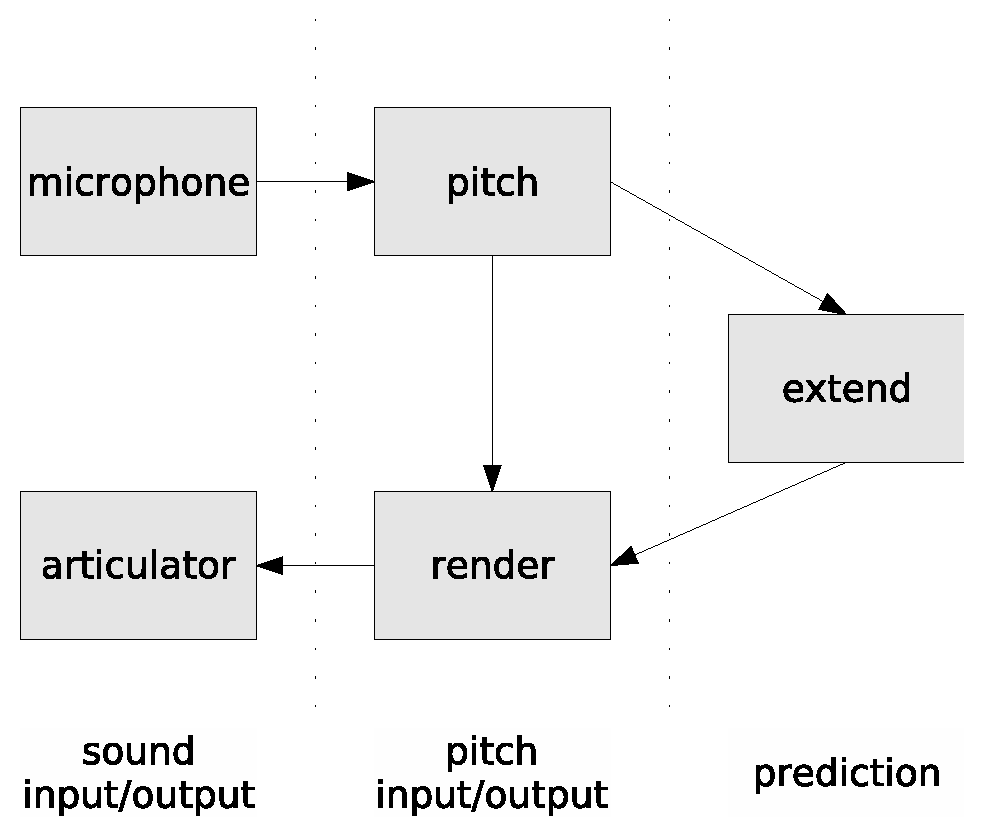
\includegraphics[height=6cm]{images/sing-modules}}
\caption {
%
The system for vocal interaction.
The behavior is implemented in the module labelled {\bf render} which
takes the output both of the pitch detector ({\bf pitch}) and a simultaneous 
prediction of what the pitch ``ought'' to be (from {\bf extend})
and decides what sound to make if any.
%
}
\end{figure}


\subsection{Implementation}

Work has now been applied in practice, as a proof-of-concept.

 to a pitch
perception/production experiment.  We attached prediction to the
property of acoustic pitch.


- Apply across multiple signals

- Different aspects of speech sounds

- Arm movements, gesturing

- Exploit knowledge of structure for learning of parts


\subsection{Summary}

(spectrograms just show a low frequency range, to make the pitch visible).

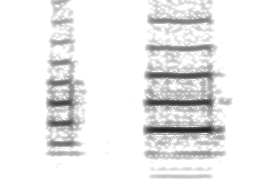
\includegraphics[height=2cm]{images/chico-output-separate-high-low}

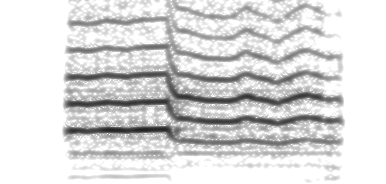
\includegraphics[height=2cm]{images/chico-output-pair-high-low}

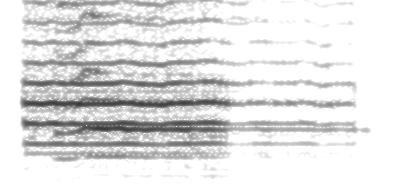
\includegraphics[height=2cm]{images/chico-output-ohm}

\subsection{Tone sequence}

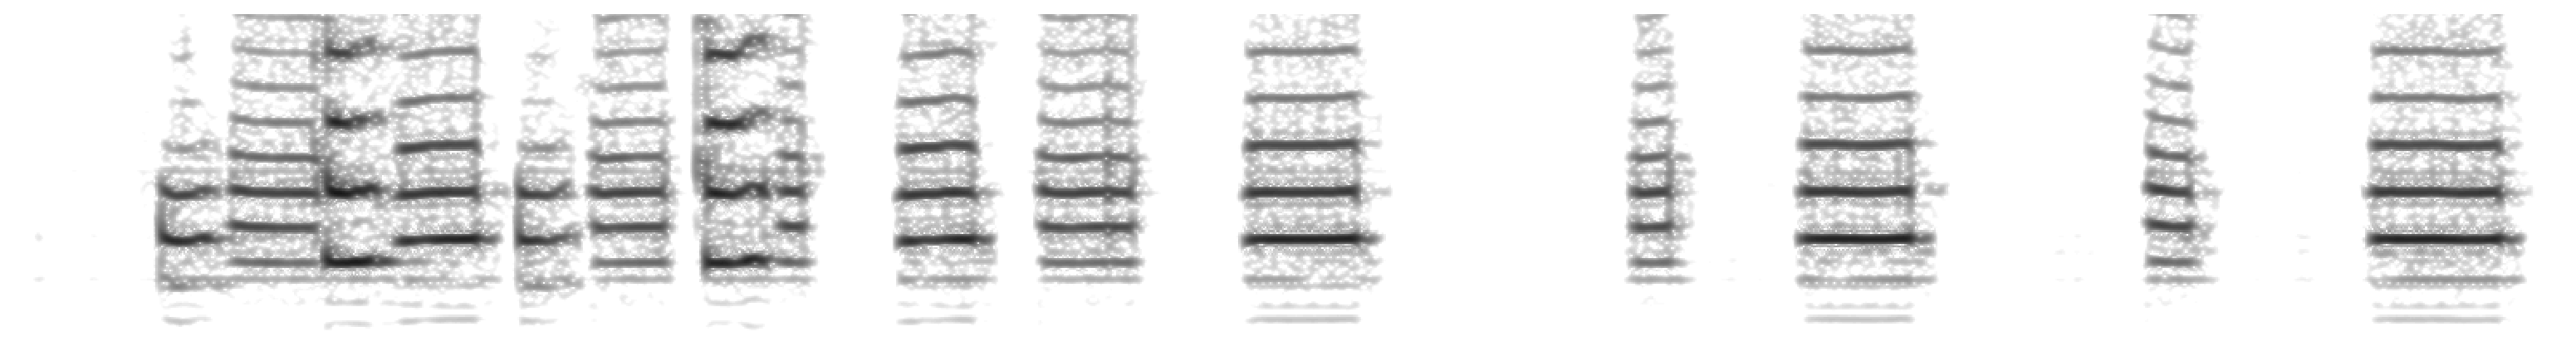
\includegraphics[height=2cm]{images/chico-separate-begin}

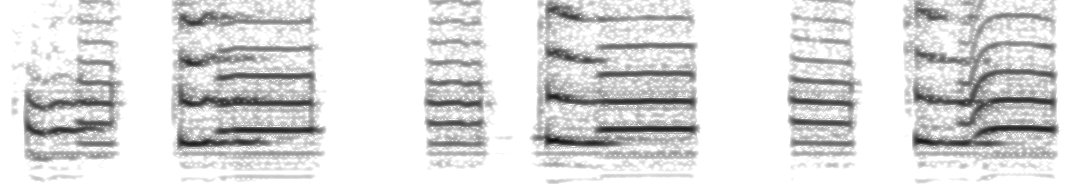
\includegraphics[height=2cm]{images/chico-separate-together}

\subsection{Prosodic unit}

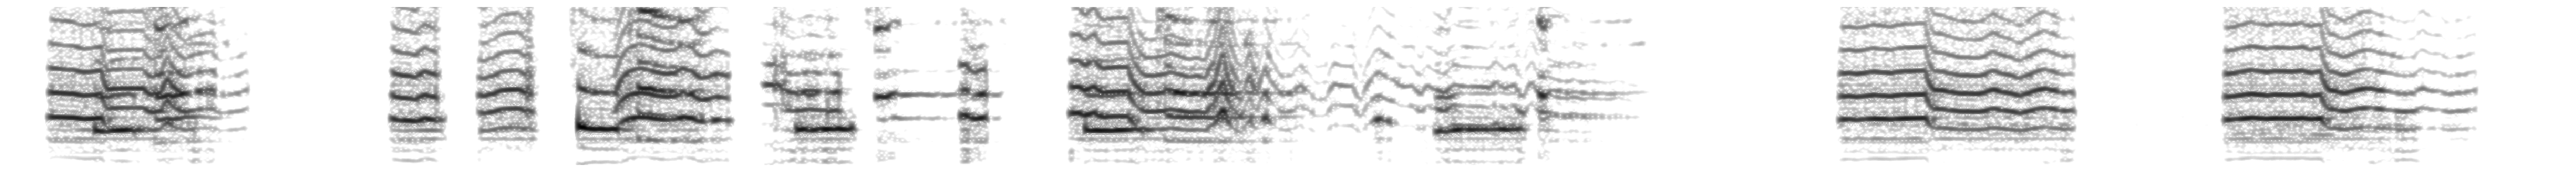
\includegraphics[height=1cm]{images/chico-pair}

\subsection{Ohm}

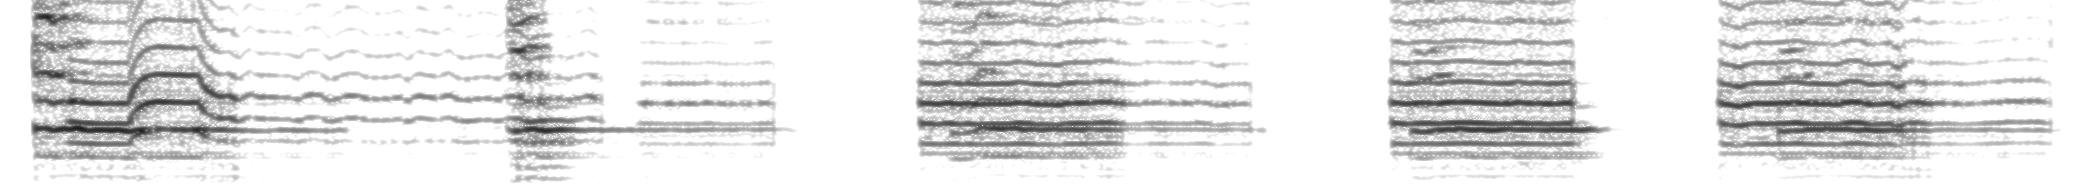
\includegraphics[height=1cm]{images/chico-ohm}




